\documentclass[10pt,a4paper]{article}
\usepackage[utf8]{inputenc}
\usepackage[T1]{fontenc}
\usepackage{url}
\usepackage{amsmath}
\usepackage{amsfonts}
\usepackage{amssymb}
\usepackage{graphicx}
\usepackage{caption}
\usepackage{subcaption}
\usepackage{xcolor}
\setlength{\parindent}{0cm}

\begin{document}
	\begin{titlepage}
		\begin{center}
			\vspace*{1cm}
			
			\Huge{\textbf{Omnibot}}
			
			\vspace{0.5cm}
			Process Documentation
			
			
			\vfill
			
			
			
			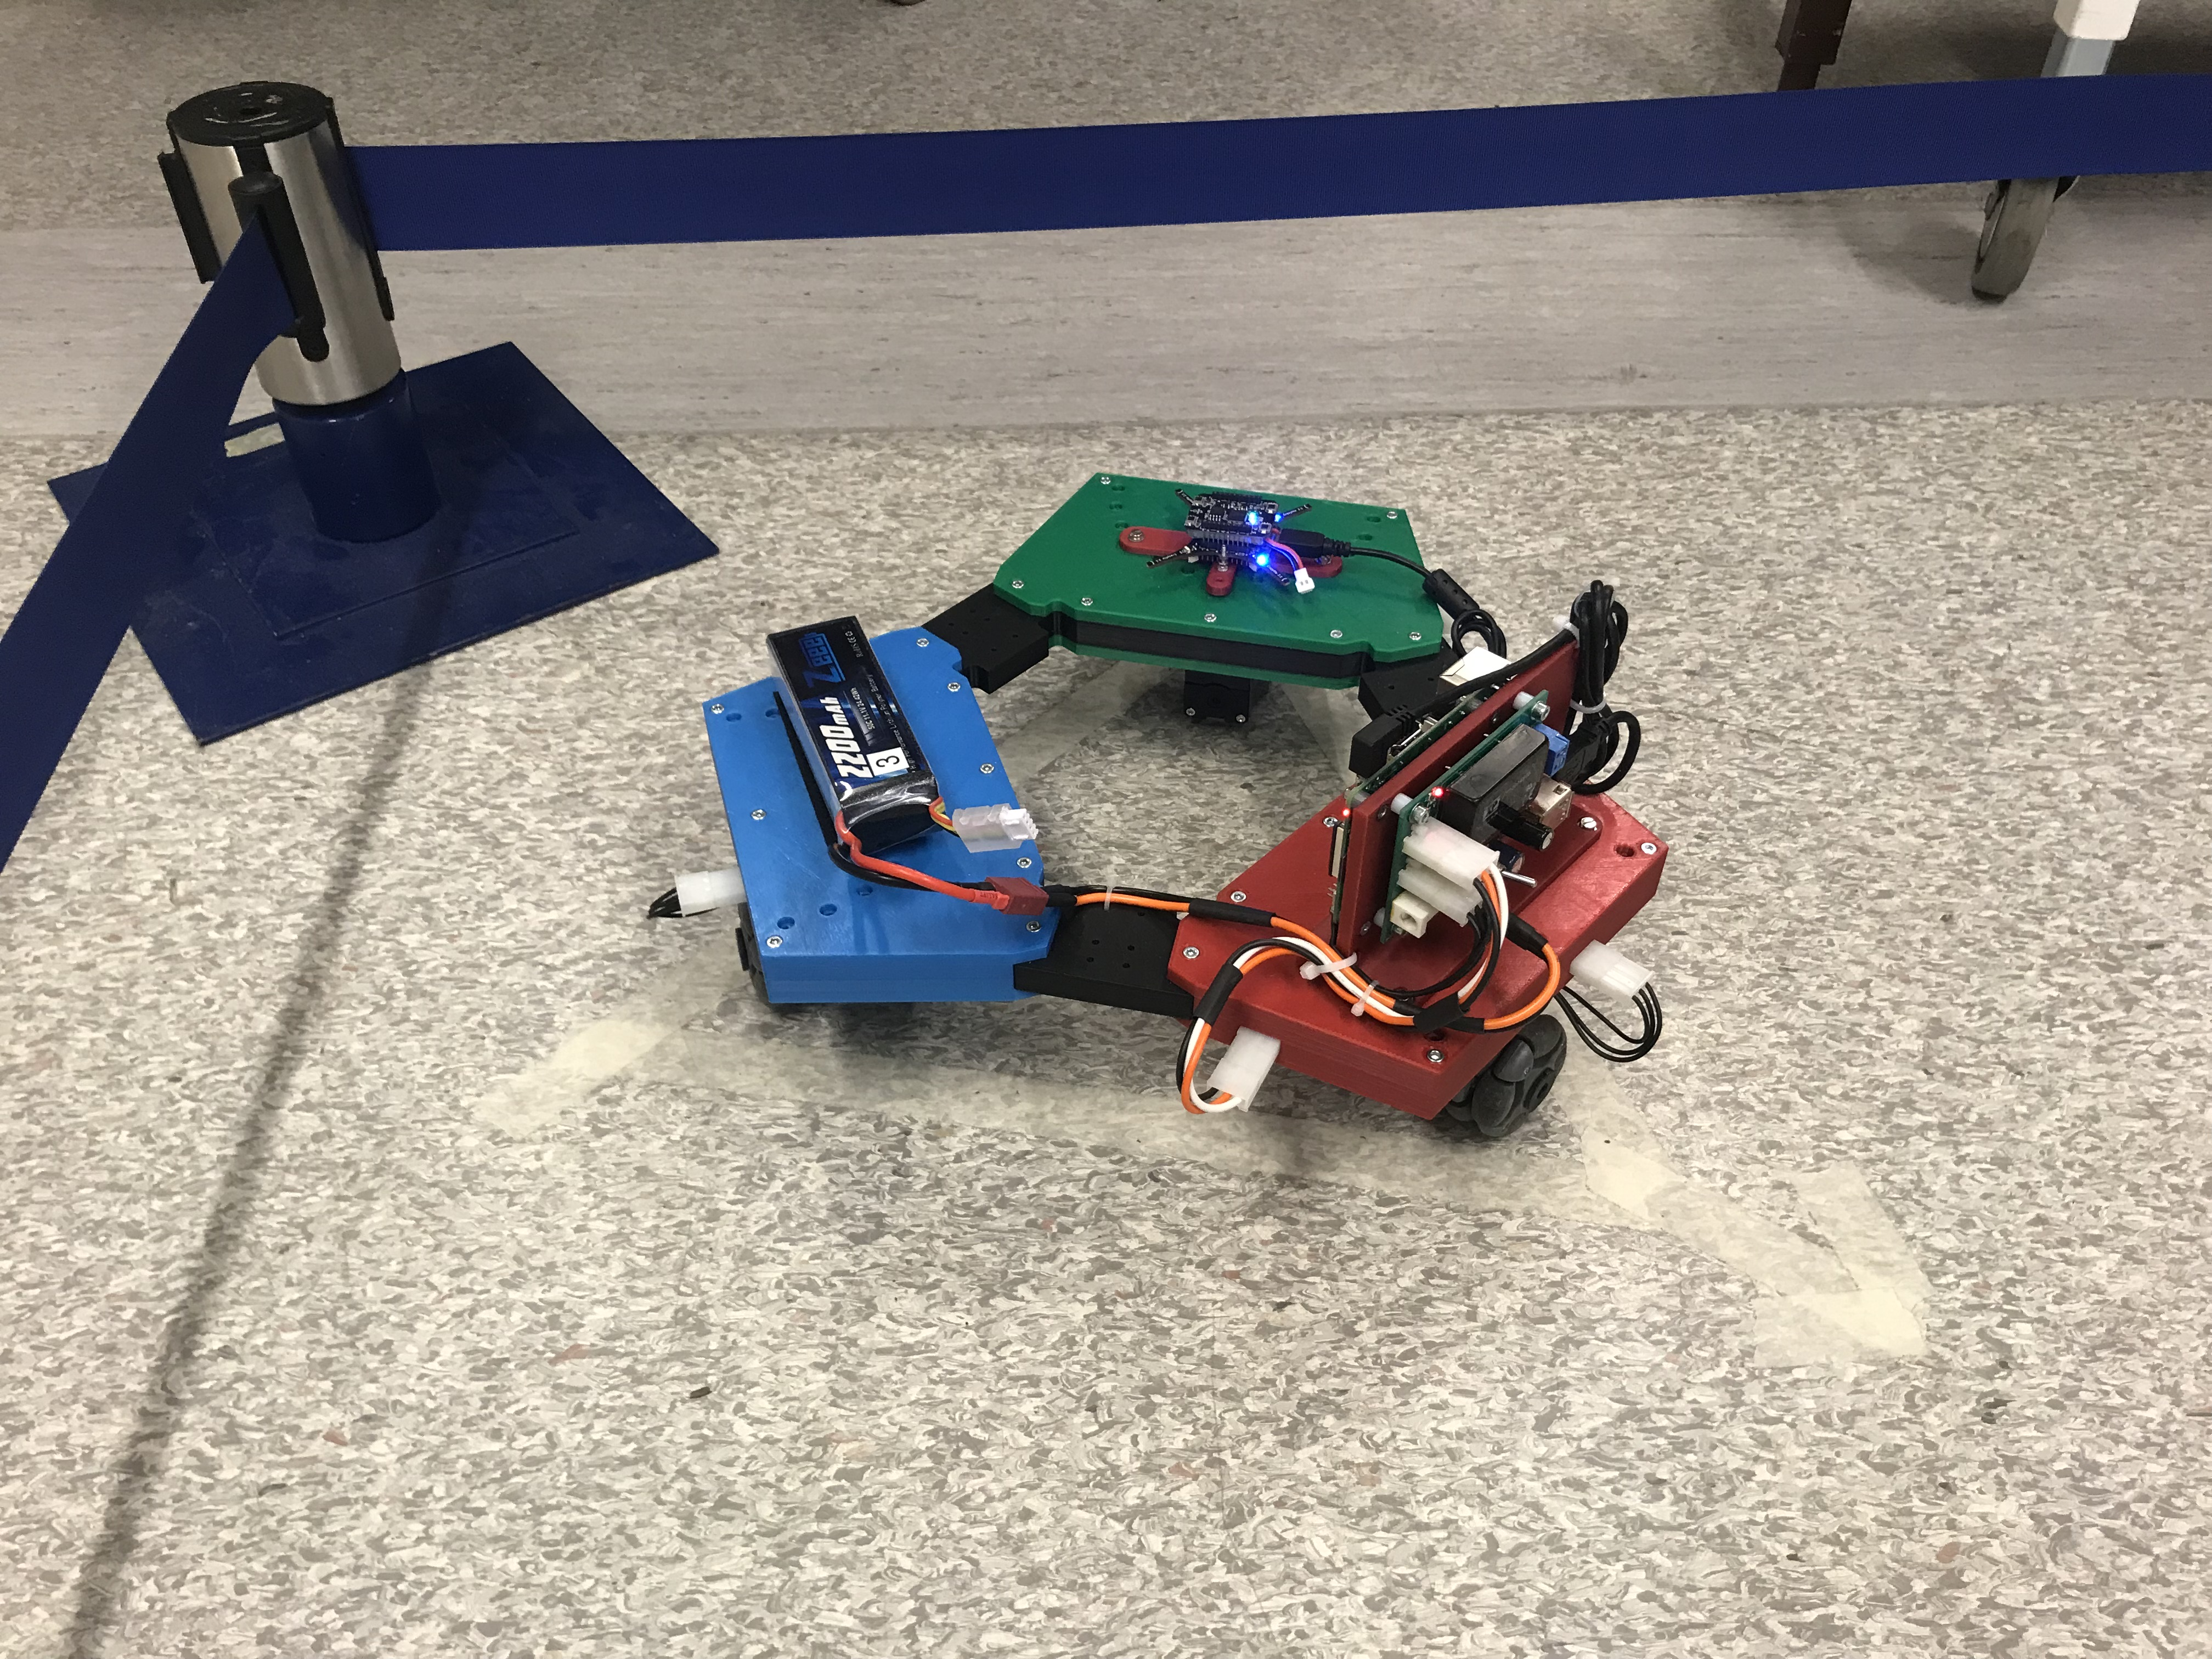
\includegraphics[width=\textwidth]{figs/bot.jpg}
			\vspace{0.8cm}
			
		\end{center}
	\end{titlepage}
	
	\section{Background}
	The omnibot is a robot mounted with omni wheels, allowing it to traverse in any given direction. There have been a few projects run on the omnibot. The base was 3d-printed by Anders Blomdell, who also attached the dynamixel servos and wheels. Mounts and power supply was managed by Alexander Pisarevskiy.
	
	\subsection{MAX 4 project}
	A masters project has been done in using the omnibots, along with a mounted delta robot, to draw floor markings. An overview of this project can be found in the file \textit{MAX4\_project\_report.pdf}.
	
	\subsection{FRTN75 lab}
	In the course FRTN75, a motion planning lab was held with the omnibot. Here we pretended that the robot could only move in accordance to car dynamics. The lab can be found by logging into any of the lab computers \textit{philon-xx.control.lth.se} where xx is e.g. 04, a number between 1 and 12, through a browser. Then going into the frtn75-planning lab on the jupyterhub server.
	
	\section{General Description}
	
	\section{Robot Dynamics}
	In the MAX4 project, the connection between wheel rotational speed and robot translational and rotational speed. See the file \textit{MAX4\_project\_report.pdf} for more details. The results are summarized here, and illustrated in Figure \ref{fig:dynamics}.
	
	\begin{figure}[h]
		\centering
		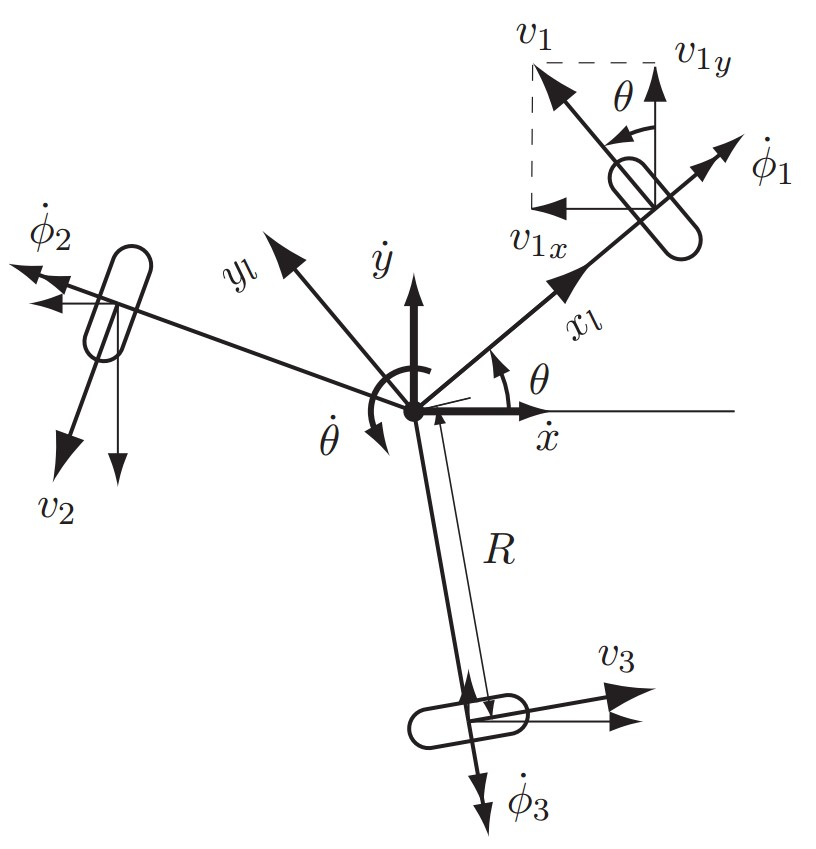
\includegraphics[width=0.4\textwidth]{figs/dynamics}
		\caption{Robot dynamics. Image stolen from \textit{MAX4\_project\_report.pdf}}
		\label{fig:dynamics}
	\end{figure}

	Given coordinates $x$, $y$ and rotation $\theta$ in a global coordinate system and wheels labelled 1, 2 and 3. The connection between $\dot{x}$, $\dot{y}$ and $\dot{\theta}$ and the rotational speed of the wheels, $\dot{\phi}_1$, $\dot{\phi}_2$ and $\dot{\phi}_3$ is
	
	\begin{equation}
		\begin{pmatrix}
			\dot{\phi}_1 \\ \dot{\phi}_2 \\ \dot{\phi}_3
		\end{pmatrix} = \frac{1}{r}\begin{pmatrix}
		-\sin(\theta) & \cos(\theta) & R \\
		-\sin(\theta +2\pi/3) & \cos(\theta +2\pi/3) & R \\
		-\sin(\theta +4\pi/3) & \cos(\theta +4\pi/3) & R \\
		\end{pmatrix} \begin{pmatrix}
			\dot{x} \\ \dot{y} \\ \dot{\theta}
		\end{pmatrix}
	\end{equation}
	Here $R$ is the distance from the center of the robot to the wheels, and $r$ is the radius of the omniwheels.
	
	\section{Crazyflie Positioning}
	
	A crazyflie (version $\geq$ 2.0) has been used to provide positioning for the robot. This is done via a lighthouse deck (\url{https://www.bitcraze.io/products/lighthouse-positioning-deck/}) mounted on the crazyflie, along with HTC vive beacons mounted in the ceiling above the robot (\ref{fig:beacon}). 
	
	\begin{figure}[h]
		\centering
		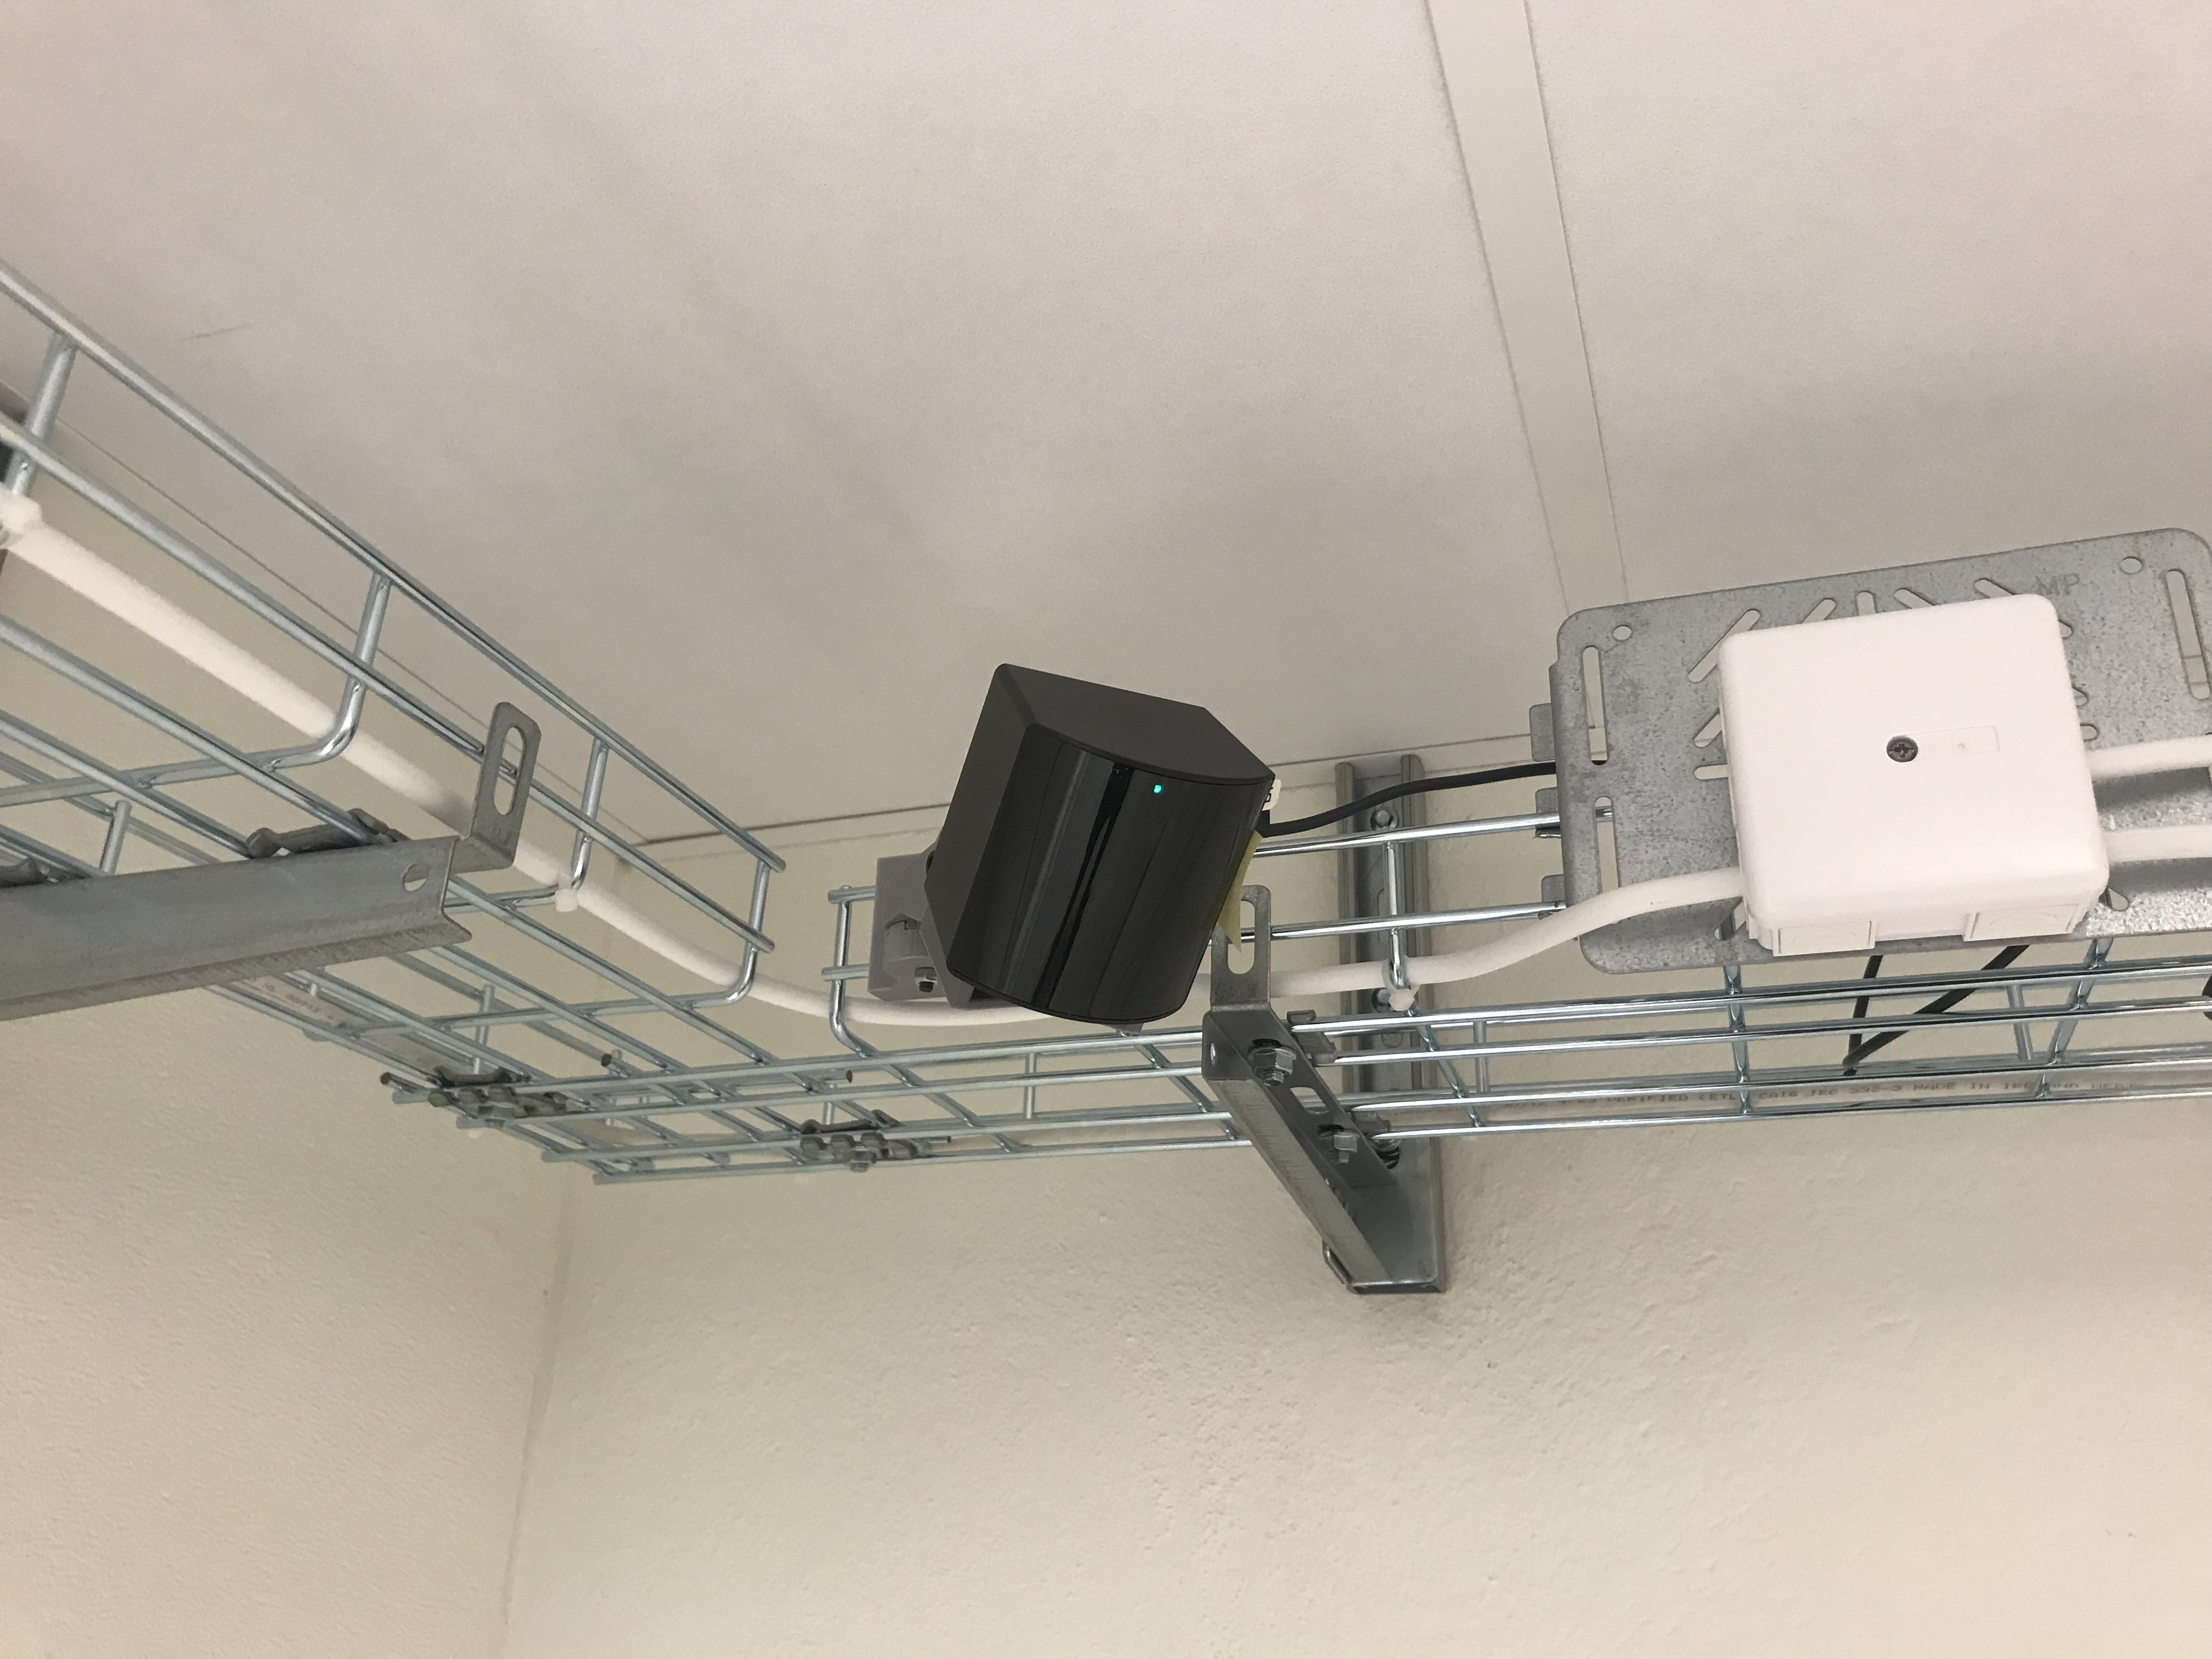
\includegraphics[width=0.7\textwidth]{figs/beacon}
		\caption{HTC vive positioning system.}
		\label{fig:beacon}
	\end{figure}
	
	\subsection{Setting up the crazyflie}
		When setting up the robot, make sure the crazyflie firmware is up to date, along with the firmware on the lighthouse deck. To update the version, use an external laptop together with a crazyradio and the crazyflie client (pip install cfclient).
		\\
		
		\textbf{Crazyradio}: \url{https://www.bitcraze.io/products/crazyradio-pa/}\\
		\textbf{Cfclient}: \url{https://www.bitcraze.io/documentation/repository/crazyflie-clients-python/master/userguides/userguide_client}
		\\
		
		To be able to connect to the crazyflie, make sure you have the right USB permissions: \url{https://www.bitcraze.io/documentation/repository/crazyflie-lib-python/0.1.9/usb_permissions/}
		\\
		
		Once you have the crazyflie client up and running, update to the latest firmware. To do this, you must use a crazyradio to connect to the crazyflie, and the crazyflie must be connected to a battery (sadly it doesn't work to just connect to it via usb). You will find firmware update instructions here:
		\url{https://www.bitcraze.io/documentation/repository/crazyflie-clients-python/master/userguides/userguide_client/#firmware-upgrade}
		
		Once the firmware has been updated, you will not need the battery again.
		
	\subsection{Setting up lighthouse system}
		The beacons are mounted via 3d-printed mounts. See the 3Dprint-folder for models. Instructions on how to configure the lighthouse system can be found here:
		\url{https://www.bitcraze.io/documentation/tutorials/getting-started-with-lighthouse/}
		
		
	\subsection{Connecting to raspberry pi}
		The raspberry pi is connected to the crazyflie via USB, which provides both power and communication. If you notice that the crazyflie turns on, but you cannot establish connection via the USB, try switching USB cables. Some USB cables don't transfer data.
	
	\subsection{Reconfigure coordinate system}
		Before you start running the robot, you will have to configure the robot's coordinate system. This is most easily done by connecting to the crazyflie via an external laptop using the crazyradio dongel and the crafyflie client. Instructions can be found here:
		\url{https://www.bitcraze.io/documentation/tutorials/getting-started-with-lighthouse/}
		\\
		
		Note that the coordinate system doesn't need to be reconfigured everytime you boot up the crazyflie. However, if you make any changes like moving your beacons or testing area you will have to do this step.
		
	\section{Dynamixel Servos}
	
	The interface between the raspberry pi and the dynamixel servos driving the wheels is developed by Anders Blomdell in the form of a python package that can be found here:
	\url{https://gitlab.control.lth.se/anders_blomdell/dynamixel}
	\\
	
	The servos have several important settings. When writing a script to control the robot, it is important to know the channel number and communication speed of each servo. The easiest ways to check or change the current settings on the servos is by downloading the dynamixel wizard to a laptop, and connecting the servos to the laptop. The wizard also allows changing the maximum set-speed of the servos.
	\url{https://emanual.robotis.com/docs/en/software/dynamixel/dynamixel_wizard2/}
	
	\section{Raspberry Pi}
	The Raspberry Pi needs very little preparation. In the FRTN75-setup, it was booted with a simple raspian distribution. Instructions for setting up a raspberry pi with raspian:
	\url{https://www.raspberrypi.com/documentation/computers/getting-started.html}
	\textbf{Make sure to change the default password of the raspberry pi before connecting it to the internet!}
	\\
	
	In the FRTN75-course, a few python packages were needed, listed in \textit{requirements.txt} in the \textit{code} folder. Note that the python-dynamixel package is not available from pip, but needs to be pip-installed from the gitlab-repository you find under the \textit{dynamixel servos} section.
	\\
	
	In order to allow the raspberry pi to communicate with the crazyflie, you need to ensure the right USB settings. Instructions for this are available under the \textit{Crazyflie positioning} section.
	\\
	
	If the communication method of choice is ssh, as in the FRTN75-course, make sure SSH is enabled on the raspberry pi.
	
	
	\section{Frame and Power Supply}
	
	The frame was designed and 3d-printed by Anders Blomdell. Alexander Pisarevskiy designed and printed the mounts for the power supply, raspberry pi and crazyflie. 3D-print designs can be found in the \textit{3Dprint}-folder.
	\\
	
	The robot can be fed either through battery or cable. When the cable is connected it overrides the battery supply. During the FRTN75-labs, only the battery supply was used. One battery would last around two lab sessions à 4 hours, but in each session the robot was only on and running for around 1 hour in total.
	\\
	
	The batteries are charged with the charging system in Figure \ref{fig:charger}.
	
	\begin{figure}[h]
		\centering
		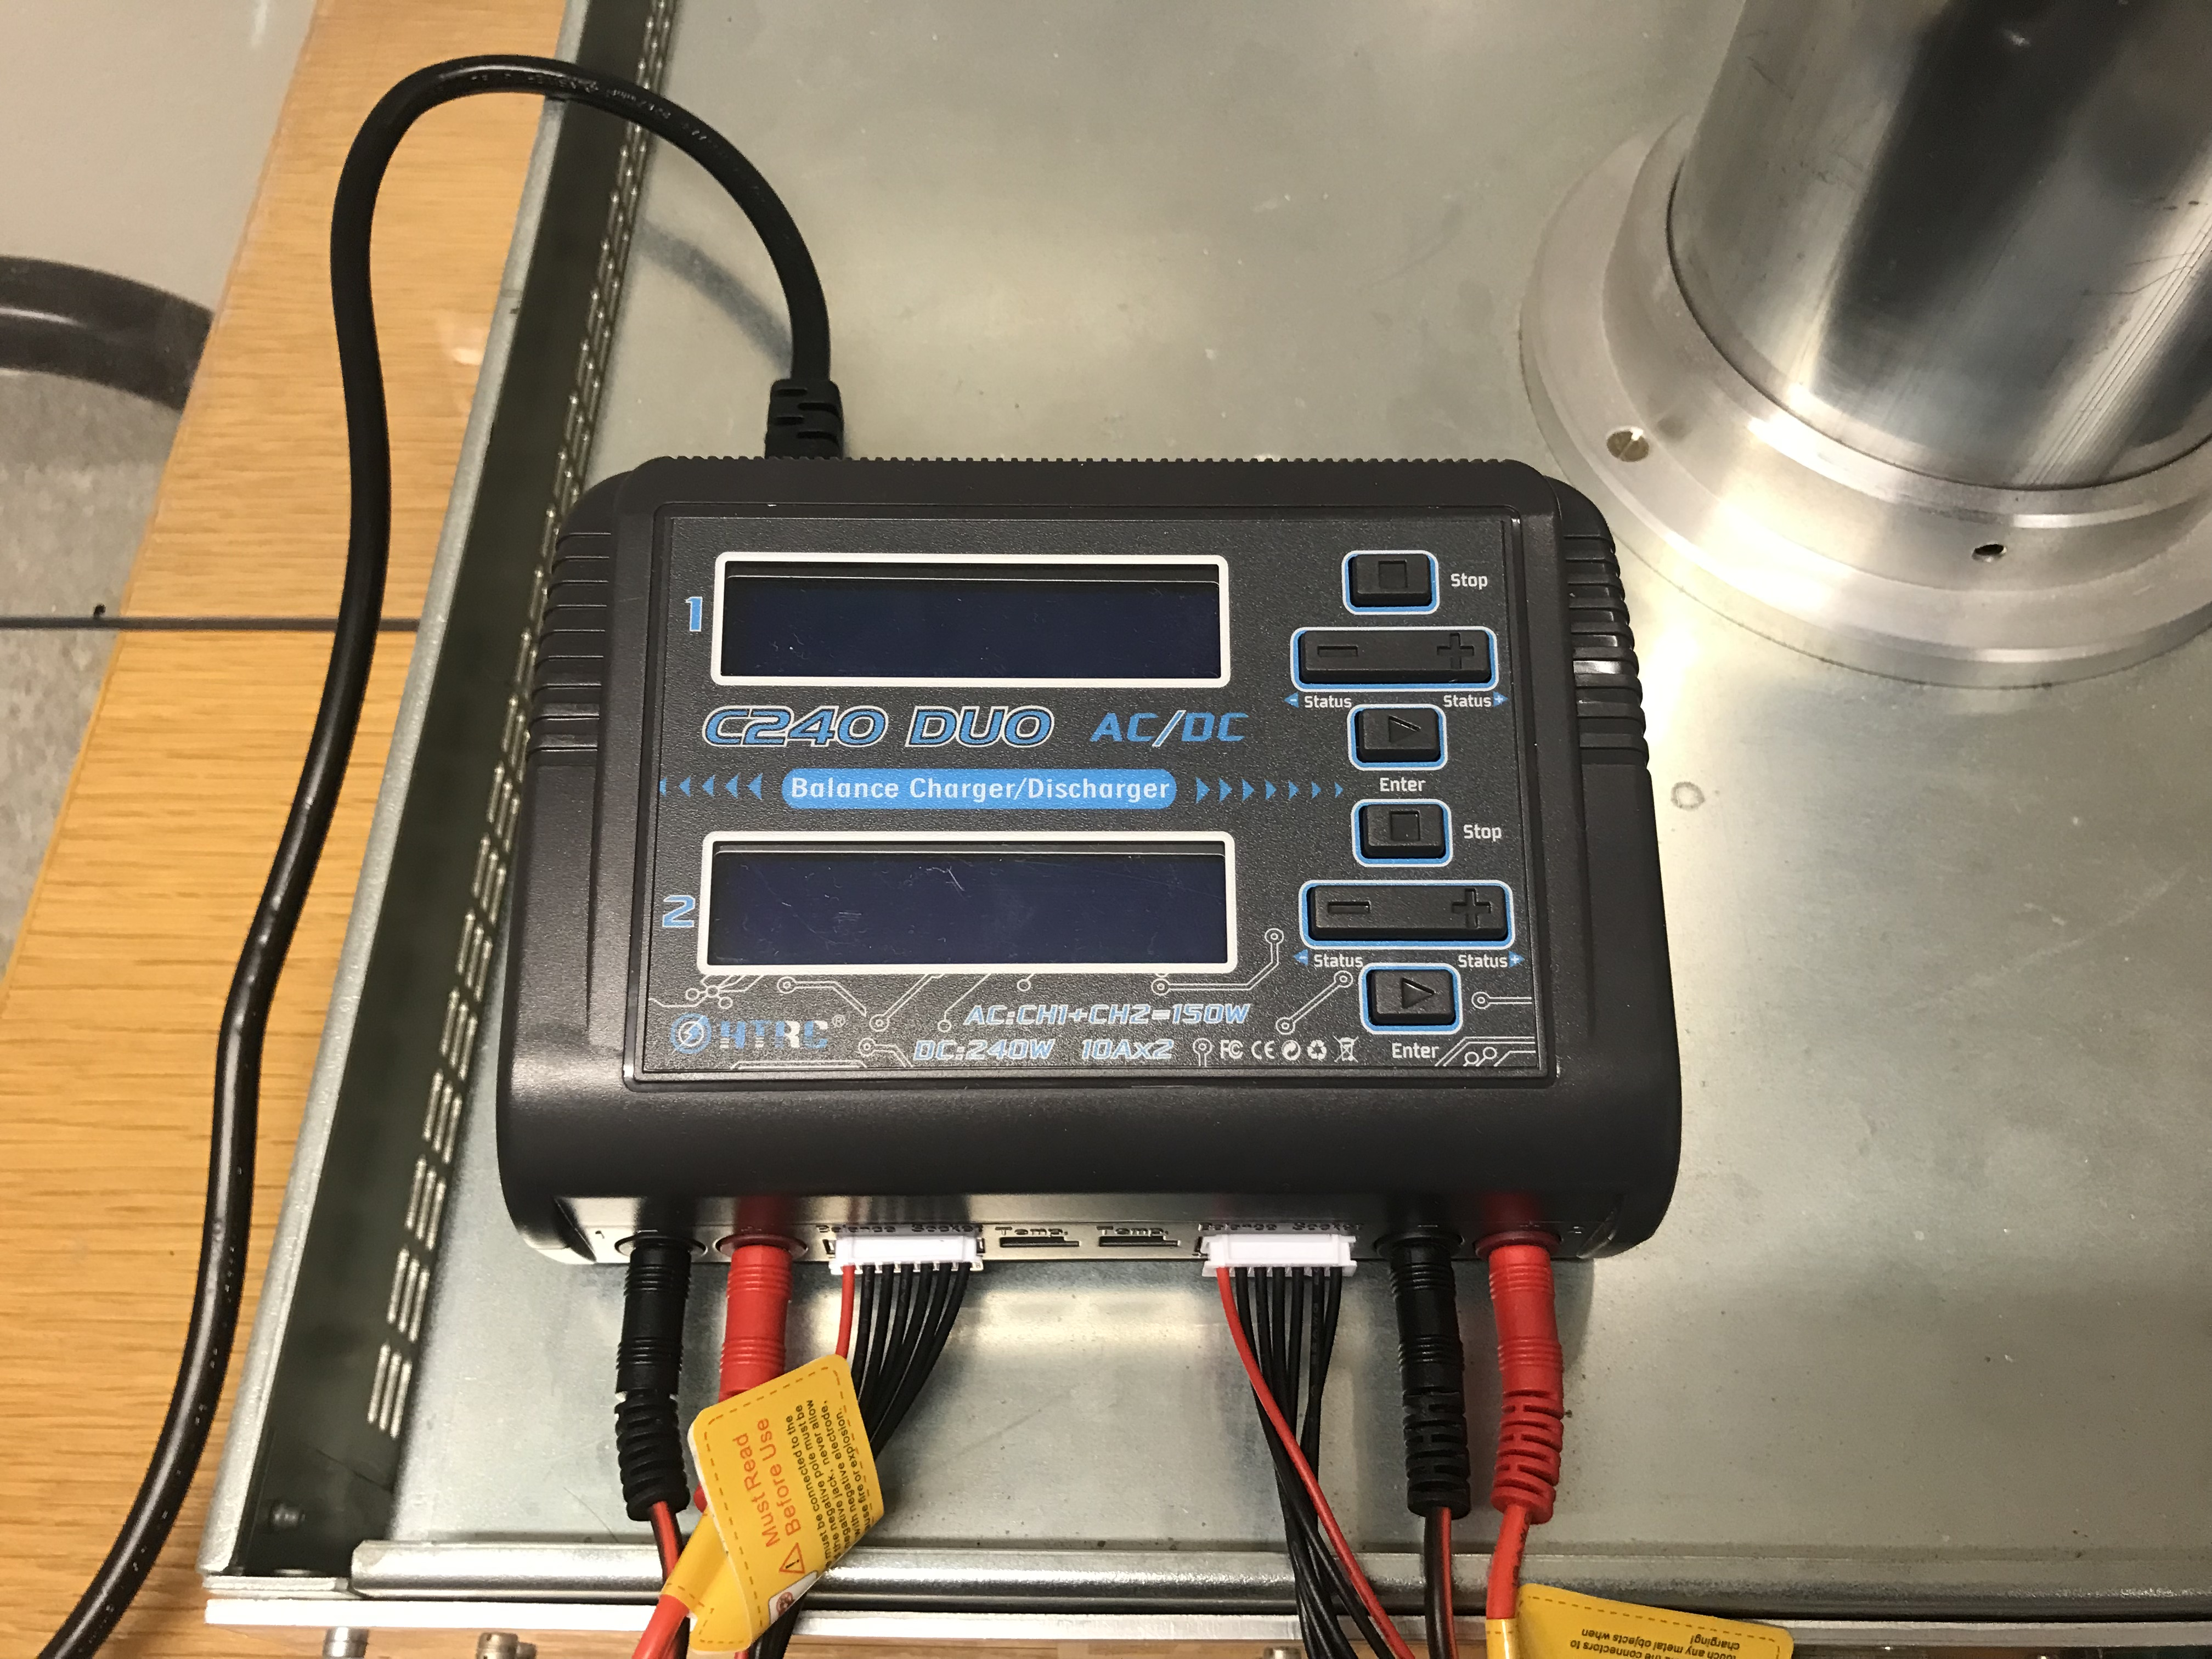
\includegraphics[width=0.7\textwidth]{figs/charger}
		\caption{Battery charging system.}
		\label{fig:charger}
	\end{figure}

	\section{Communication}
	In the FRTN75 course, there was no online communication between the raspberry pi and external computers. A local router was set up in the lab, where the raspberry pi was given a static IP address. This allowed students to ssh into the device to leave a reference trajectory file (csv format), and then execute the script \texttt{track\_path.py}, which read the file and executed it.
	
	\section{Code and Scripts}
	
	
	
	\url{https://gitlab.control.lth.se/anders_blomdell/dynamixel}
\end{document}
